\documentclass[a4paper]{article}

%%%%%%%% CREATE DOCUMENT STRUCTURE %%%%%%%%
%% Language and font encodings
\usepackage[polish]{babel}
\usepackage[utf8]{inputenc}
\usepackage[T1]{fontenc}
%\usepackage{subfig}

%% Sets page size and margins
\usepackage[a4paper,top=3cm,bottom=2cm,left=2cm,right=2cm,marginparwidth=1.75cm]{geometry}

%% Useful packages
\usepackage{amsmath}
\usepackage{graphicx}
\usepackage[colorinlistoftodos]{todonotes}
\usepackage{float}
\usepackage[colorlinks=true, allcolors=blue]{hyperref}
\usepackage{caption}
\usepackage{subcaption}
\usepackage{sectsty}
\usepackage{titling}
\usepackage{blindtext}
\usepackage[square,sort,comma,numbers]{natbib}
\usepackage[colorinlistoftodos]{todonotes}
\usepackage{xcolor}
\definecolor{darkgreen}{rgb}{0.0, 0.4, 0.0}

%%%%%%%% DOCUMENT %%%%%%%%
\begin{document}

%%%% Title Page
\begin{titlepage}

\newcommand{\HRule}{\rule{\linewidth}{0.5mm}}
\center

\textsc{\LARGE Politechnika Krakowska}\\[1cm]

\textsc{\Large Bezpieczeństwo i Hardening Systemów Operacyjnych}\\[0.2cm]
\HRule \\[0.8cm]
{ \huge \bfseries Szyfrowanie danych w systemie Linux: analiza porównawcza LUKS, eCryptfs i fscrypt }\\[0.7cm]
\HRule \\[2cm]
\Large Jakub Mikusek\\[1.5cm]
{\large \today}\\[5cm]
% \includegraphics[width=0.5\textwidth]{PK_logo.png}\\[1cm]
\vfill
\end{titlepage}

\section{Wprowadzenie}
Szyfrowanie danych stanowi jeden z fundamentalnych elementów ochrony informacji w systemach
komputerowych. W środowiskach Linux dostępnych jest kilka mechanizmów szyfrowania, różniących
się poziomem abstrakcji, sposobem zarządzania kluczami oraz charakterystyką wydajnościową.
Analiza obejmuje trzy rozwiązania: LUKS (Linux Unified Key Setup), realizujący szyfrowanie
na poziomie urządzenia blokowego za pośrednictwem dm-crypt; eCryptfs, będący kryptograficznym
systemem plików działającym jako nakładka na zwykły system plików, oraz fscrypt, zintegrowany
bezpośrednio z systemem plików na poziomie jądra. Każde z tych rozwiązań oferuje odmienny model
bezpieczeństwa, inaczej reaguje na zagrożenia offline i online, a także wykazuje różną
charakterystykę wydajnościową w zależności od specyfiki operacji wyjścia/wejścia.
\\\\
W ramach projektu stworzony został benchmark porównujący wydajność każdego ze wspomnianych
mechanizmów, porównanie oraz sposób działania każdego z nich oraz rekomendacje dla scenariuszy
użycia.


\section{Wybrane mechanizmy szyfrowania plików}

\subsection{LUKS - Linux Unified Key Setup}
Jest to sposób szyfrowania dysków, domyślnie przeznaczony dla systemów Linux. Szyfrowanie
za pomocą LUKS opiera się na szyfrowaniu urządzeń blokowych (ang. block device). Pozwala to
na zaszyfrowanie dowolnego systemu plików, uwzględniając partycje SWAP. LUKS stanowi warstwę
zarządzania kluczami dla dm-crypt, zapewniając standaryzowany format nagłówka na urządzeniu.
Każdy z zaszyfrowanych wolumenów zawiera niezaszyfrowany nagłówek, który w wersji LUKS2
pozwala na przechowywanie do 32 kluczy dostępu do danych. Szyfrowanie danych w ramach LUKS
jest wieloetapowe. Klucz główny szyfruje dane, a klucze użytkowników szyfrują klucz główny,
co pozwala na zmiany kluczy poszczególnych użytkowników bez konieczności ponownego szyfrowania
wszystkich danych. Szyfrowanie całych partycji pozwala na zaszyfrowanie kluczowych elementów
systemu operacyjnego oraz na automatyczne deszyfrowanie danych podczas uruchamiania systemu
operacyjnego. Szyfrowanie całych partycji charakteryzuje się niewielkim narzutem związanym
z zapisem oraz odczytem danych.

\subsubsection{Model zagrożeń i ochrona}
LUKS zapewnia pełną ochronę poufności danych w przypadku ataków offline, takich jak fizyczna
kradzież dysku lub dostęp do odmontowanej partycji zaszyfrowanej, pod warunkiem użycia silnego
hasła lub klucza. W scenariuszu offline atakujący nie ma dostępu do odszyfrowanych danych bez
znajomości co najmniej jednego z kluczy użytkownika. Nagłówek LUKS, choć niezaszyfrowany,
zawiera jedynie metadane kryptograficzne i zaszyfrowane kopie klucza głównego.
Warto jednak zwrócić uwagę, że zniszczenie nagłówka LUKS uniemożliwia odzyskanie danych,
nawet przy znajomości hasła.

W przypadku ataków online, gdy partycja LUKS jest zmontowana i aktywnie używana, wszystkie
dane są dostępne dla procesów mających odpowiednie uprawnienia w systemie. LUKS nie zapewnia
ochrony przed złośliwym oprogramowaniem działającym z uprawnieniami root, ani przed atakami
na działający system. Ataki \textit{cold boot}, polegające na odczytaniu zawartości pamięci
RAM krótko po wyłączeniu zasilania, mogą ujawnić klucz główny dm-crypt, który jest przechowywany
w pamięci jądra podczas gdy partycja jest zamontowana.


\subsection{eCryptfs}
eCryptfs  w odróżnieniu od pozostałych użytych mechanizmów szyfrowania, jest kryptograficznym
systemem plików działającym jako nakładka na istniejący system plików, natywnie wspieranym
przez Linux. Pozwala on na szyfrowanie per-plik na poziomie systemu plików, bez konieczności
tworzenia dedykowanego zaszyfrowanego wolumenu. Dzięki temu eCryptfs może zostać zamontowany
w dowolnym katalogu.

Każdy plik szyfrowany jest przy użyciu losowo generowanego klucza, który jest przechowywany
zaszyfrowany w nagłówku pliku. eCryptfs wspiera swobodny dostęp, co pozwala na niezależne
przenoszenie i odszyfrowywanie poszczególnych plików bez konieczności dostępu do centralnego
magazynu kluczy.

Mechanizm ten niesie jednak za sobą szereg istotnych ograniczeń. Zaszyfrowane pliki są zawsze
większe niż oryginały ze względu na kryptograficzny nagłówek. Ponadto, szyfrowanie
nazw plików wymaga ich zakodowania przy użyciu uuencode, co ogranicza maksymalną długość
nazwy pliku z 255 bajtów do 143 bajtów. Warto dodać, że eCryptfs nie jest aktywnie rozwijany
od 2016 roku i projekt jest uznawany za przestarzały (m.in. Ubuntu oficjalnie wycofało go
jako mechanizm szyfrowania katalogów domowych).

\subsubsection{Model zagrożeń i ochrona}
eCryptfs zapewnia poufność zawartości plików oraz przy włączonej opcji
\texttt{ecryptfs\_enable\_filename\_crypto} również nazw plików. W scenariuszach ataku
offline, takich jak fizyczny dostęp do nośnika danych lub kradzież urządzenia.
Ponieważ metadane kryptograficzne przechowywane są w nagłówku każdego pliku, ochrona jest
zachowana nawet przy przeniesieniu pojedynczego pliku na inny nośnik, ponieważ
odszyfrowanie wymaga znajomości klucza głównego użytkownika.

Jednakże eCryptfs nie chroni metadanych systemu plików. Uprawnienia oraz struktura katalogów
są widoczne bez uwierzytelnienia. Atakujący posiadający fizyczny dostęp do nośnika może uzyskać
informacje o liczbie i przybliżonych rozmiarach plików, a bez włączonego szyfrowania nazw,
również ich pełne nazwy. Należy ponadto zaznaczyć, że eCryptfs nie zapewnia ochrony integralności
ani autentyczności danych. Brakuje mu wbudowanych mechanizmów wykrywania celowej modyfikacji
zaszyfrowanych plików.

W kontekście ataków online, gdy katalog eCryptfs jest zamontowany, wszystkie procesy
posiadające odpowiednie uprawnienia systemowe mają dostęp do odszyfrowanych danych.
eCryptfs nie zapewnia ochrony przed złośliwym oprogramowaniem działającym z uprawnieniami
root. Klucze szyfrowania są przechowywane w przestrzeni kluczy jądra,  co oznacza, że ataki
\textit{cold boot} lub kompromitacja pamięci jądra mogą prowadzić do ich ujawnienia i tym samym
do utraty poufności wszystkich plików z odszyfrowanego katalogu.


\subsection{fscrypt}
W przeciwieństwie do dm-crypt, fscrypt działa na poziomie systemu plików. Dzięki temu
wykorzystanie tego mechanizmu szyfrowania pozwala na niezależne szyfrowanie pojedynczych
plików. Taki sposób szyfrowania daje większą elastyczność oraz w przypadku urządzeń
wykorzystywanych przez wielu użytkowników, pozwala na logiczny podział odstępu do
poszczególnych plików.

Bezpośrednie zintegrowanie fscrypt do systemu plików pozwala na lepszą wydajność,
w porównaniu do eCryptfs, gdzie jest on dodatkową abstrakcją na system plików. Takie
podejście pozwala na szybszy dostęp do zawartości plików, bez konieczności przechowywania
w pamięci podręcznej zaszyfrowanej oraz odszyfrowanej wersji pliku. Dodatkową zaletą
używania fscrypt w stosunku do eCryptfs jest brak narzutu związanego z metadanymi w nazwie
pliku, co pozwala na wykorzystanie pełnych 255 bajtów na nazwę pliku.

\subsubsection{Model zagrożeń i ochrona}
fscrypt chroni poufność zawartości plików oraz nazw plików w przypadku ataków offline,
takich jak fizyczny dostęp do urządzenia pamięci masowej, zakładając użycie silnego klucza
szyfrującego. Mechanizm ten nie chroni jednak metadanych plików (rozmiary, uprawnienia,
znaczniki czasu) ani informacji o strukturze danych (lokalizacja bloków niezaalokowanych).
fscrypt nie gwarantuje również ochrony przed manipulacją systemu plików w trybie offline
przed autoryzowanym dostępem użytkownika.

W kontekście ataków online, fscrypt oferuje ograniczoną ochronę. Po dodaniu klucza
szyfrującego do jądra, mechanizm ten nie ukrywa zawartości ani nazw plików przed innymi
użytkownikami w systemie. Ochrona dostępu powinna być realizowana przez standardowe
mechanizmy kontroli dostępu (uprawnienia plików, ACL, LSM). Atakujący, który uzyska
możliwość odczytu pamięci jądra, może skompromitować wszystkie aktywne klucze fscrypt,
chyba że zastosowane są klucze sprzętowe (\textit{hardware-wrapped keys}). W takim przypadku
klucze główne oraz klucze szyfrowania zawartości pozostają chronione przed kompromitacją pamięci
jądra.

W przypadku pełnej kompromitacji systemu (dostęp root lub wykonanie dowolnego kodu w jądrze),
fscrypt nie zapewnia ochrony danych chronionych aktywnymi kluczami, choć klucze sprzętowe mogą
uniemożliwić eksfiltrację kluczy w formie użytecznej po wyłączeniu systemu.

\section{Wdrożenie poszczególnych mechanizmów szyfrowania}
Na potrzeby przeprowadzenia testów wydajnościowych wspomniane mechanizmy szyfrowania zostały
wdrożone w środowisku testowym składającym się z maszyny wirtualnej z systemem Ubuntu Server
24.04 LTS o parametrach:
\begin{itemize}
    \item 4GB RAM
    \item 4 rdzenie
    \item trzy partycje o rozmiarach 20 GB (partycja główna zawierająca główny system plików),
    5GB (partycja zaszyfrowana przy pomocy LUKS), 5GB (partycja przeznaczona dla fscrypt)
\end{itemize}

\subsection{LUKS}
Dla stworzenia partycji zaszyfrowanej przy pomocy LUKS, został użyty uprzednio stworzony dysk
wirtualny (/dev/sdb). Wdrożenie zaszyfrowanego wolumenu odbyło się przy pomocy następujących komend:
\begin{itemize}
    \item Wstępna inicjalizacja LUKS - \texttt{sudo cryptsetup luksFormat --type luks2 --cipher
    aes-xts-plain64 --key-size 512 --hash sha256 --pbkdf argon2id --iter-time 2000
    --verify-passphrase /dev/sdb}
    \item Otwarcie zaszyfrowanej partycji - \texttt{sudo cryptsetup open /dev/sdb luks\_test}
    \item Stworzenie systemu plików wewnątrz partycji - \texttt{sudo mkfs.ext4 -L luks\_vol
    /dev/mapper/luks\_test}
    \item Stworzenie punktu montowania dla zaszyfrowanej partycji\texttt{sudo mkdir -p
    /mnt/luks\_test}
    \item Zmontowanie zaszyfrowanego systemu plików - \texttt{sudo mount /dev/mapper/luks\_test
     /mnt/luks\_test}
\end{itemize}

\subsection{eCryptfs}
Stworzenie środowiska zawierającego zaszyfrowane pliki przy pomocy eCryptfs wymagało następujących
kroków:
\begin{itemize}
    \item Stworzenie katalogu przechowującego zaszyfrowane pliki - \texttt{sudo mkdir -p
    /mnt/ecryptfs\_encrypted}
    \item Stworzenie katalogu przeznaczonego na odszyfrowane pliki - \texttt{sudo mkdir -p
    /mnt/ecryptfs\_decrypted}
    \item Inicjalizacja eCryptfs - \texttt{sudo mount -t ecryptfs /mnt/ecryptfs\_encrypted
    /mnt/ecryptfs\_decrypted -o ecryptfs\_cipher=aes, ecryptfs\_key\_bytes=32,
    ecryptfs\_passthrough=n, \\ecryptfs\_enable\_filename\_crypto=y}
\end{itemize}

\subsection{fscrypt}
Na potrzeby stworzenia partycji obsługującej szyfrowanie za pomocą fscrypt stworzony został
dysk wirtualny /dev/sdc. Konfiguracja fscrypt wymagała następujących kroków:
\begin{itemize}
    \item Stworzenie systemu plików z obsługą fscrypt - \texttt{sudo mkfs.ext4 -O encrypt -L
    fscrypt\_vol /dev/sdc}
    \item Stworzenie punktu montowania - \texttt{sudo mkdir -p /mnt/fscrypt\_test}
    \item Zmontowanie partycji z obsługa fscrypt - \texttt{sudo mount /dev/sdc /mnt/fscrypt\_test}
    \item Inicjalizacja fscrypt na poziomie systemu Linux - \texttt{sudo fscrypt setup}
    \item Inicjalizacja wewnątrz systemu plików z obsługą fscrypt - \texttt{fscrypt setup
    /mnt/fscrypt\_test}
    \item Stworzenie katalogu, który następnie zostanie zaszyfrowany - \texttt{mkdir -p
    /mnt/fscrypt\_test/private\_data}
    \item Zaszyfrowanie uprzednio stworzonego katalogu przy pomocy fscrypt - \texttt{fscrypt
    encrypt \\
    /mnt/fscrypt\_test/private\_data --source=custom\_passphrase}
\end{itemize}

\section{Testy wydajnościowe}
Do testów porównawczych został dodatkowo zmierzony czas wykonywania operacji wejścia/wyjścia
(I/O) dla niezaszyfrowanych plików, aby w wynikach uwzględnić narzut każdej z metod szyfrowania.

Testy wydajnościowe obejmują wykorzystanie prostego polecenia \texttt{dd}, pozwalającego na
kopiowanie z oraz do plików specyfikując ilość bajtów w ramach pojedynczej operacji.
Bardziej szczegółowe testy zostały przeprowadzone przy pomocy \texttt{fio}, który pozwala
symulowanie operacji wejścia/wyjścia na podstawie zadanych parametrów.

Do automatyzacji wykonywania testów zostały stworzone dwa skrypty przy użyciu języka python3
(\textit{benchmark\_dd.py} oraz \textit{benchmark\_fio.py}). Pozwalają one dzięki
parametrom wykonania na dostosowanie ilości wykonywanych testów.

\subsection{Testy wykorzystujące \texttt{dd}}
Polecenie \texttt{dd} pozwala na proste operacje kopiowania danych pomiędzy plikami,
na podstawie zadanego rozmiaru bloku w bajtach, opcja \texttt{bs=}, oraz ilości kopiowanych
danych dzięki opcji \texttt{count=}. W połączeniu z urządzeniem \textit{/dev/urandom},
\texttt{dd} pozwala na przetestowanie przepustowości oraz szybkości kopiowania losowych danych
do plików zaszyfrowanych wybraną metodą. Natomiast wykorzystując \textit{/dev/null},
\texttt{dd} umożliwia przetestowanie szybkości kopiowania danych z plików.


\subsubsection{Wyniki uzyskane w ramach testów przy użyciu \texttt{dd}}

\begin{table}[H]
    \centering
    \begin{tabular}{|l|l|r|}
        \hline
        Mechanism & Operation & Speed (MBs) \\
        \hline
        Raw I/O [4K] & WRITE & 124.6 \\
        Raw I/O [4K] & READ & 124.4 \\
        Raw I/O [512K] & WRITE & 381.2 \\
        Raw I/O [512K] & READ & 474.9 \\
        Raw I/O [1M] & WRITE & 398.8 \\
        Raw I/O [1M] & READ & 848.5 \\
        Raw I/O [4M] & WRITE & 414.8 \\
        Raw I/O [4M] & READ & 1008.5 \\
        LUKS [4K] & WRITE & 103.39 \\
        LUKS [4K] & READ & 98.68 \\
        LUKS [512K] & WRITE & 351.1 \\
        LUKS [512K] & READ & 363.2 \\
        LUKS [1M] & WRITE & 387.1 \\
        LUKS [1M] & READ & 647.4 \\
        LUKS [4M] & WRITE & 420.3 \\
        LUKS [4M] & READ & 699.3 \\
        eCryptfs [4K] & WRITE & 94.18 \\
        eCryptfs [4K] & READ & 110.63 \\
        eCryptfs [512K] & WRITE & 210.7 \\
        eCryptfs [512K] & READ & 139.8 \\
        eCryptfs [1M] & WRITE & 218.5 \\
        eCryptfs [1M] & READ & 139.2 \\
        eCryptfs [4M] & WRITE & 217.5 \\
        eCryptfs [4M] & READ & 137.9 \\
        fscrypt [4K] & WRITE & 136.0 \\
        fscrypt [4K] & READ & 103.34 \\
        fscrypt [512K] & WRITE & 346.0 \\
        fscrypt [512K] & READ & 381.0 \\
        fscrypt [1M] & WRITE & 357.5 \\
        fscrypt [1M] & READ & 715.0 \\
        fscrypt [4M] & WRITE & 404.4 \\
        fscrypt [4M] & READ & 820.1 \\
        \hline
    \end{tabular}
    \caption{Tabela wyników operacji wyjścia (READ) oraz wejścia (WRITE) do plików w ramach
    różnych mechanizmów szyfrowania danych.}
    \label{tab:dd_results}
\end{table}

\begin{figure}[H]
    \centering
    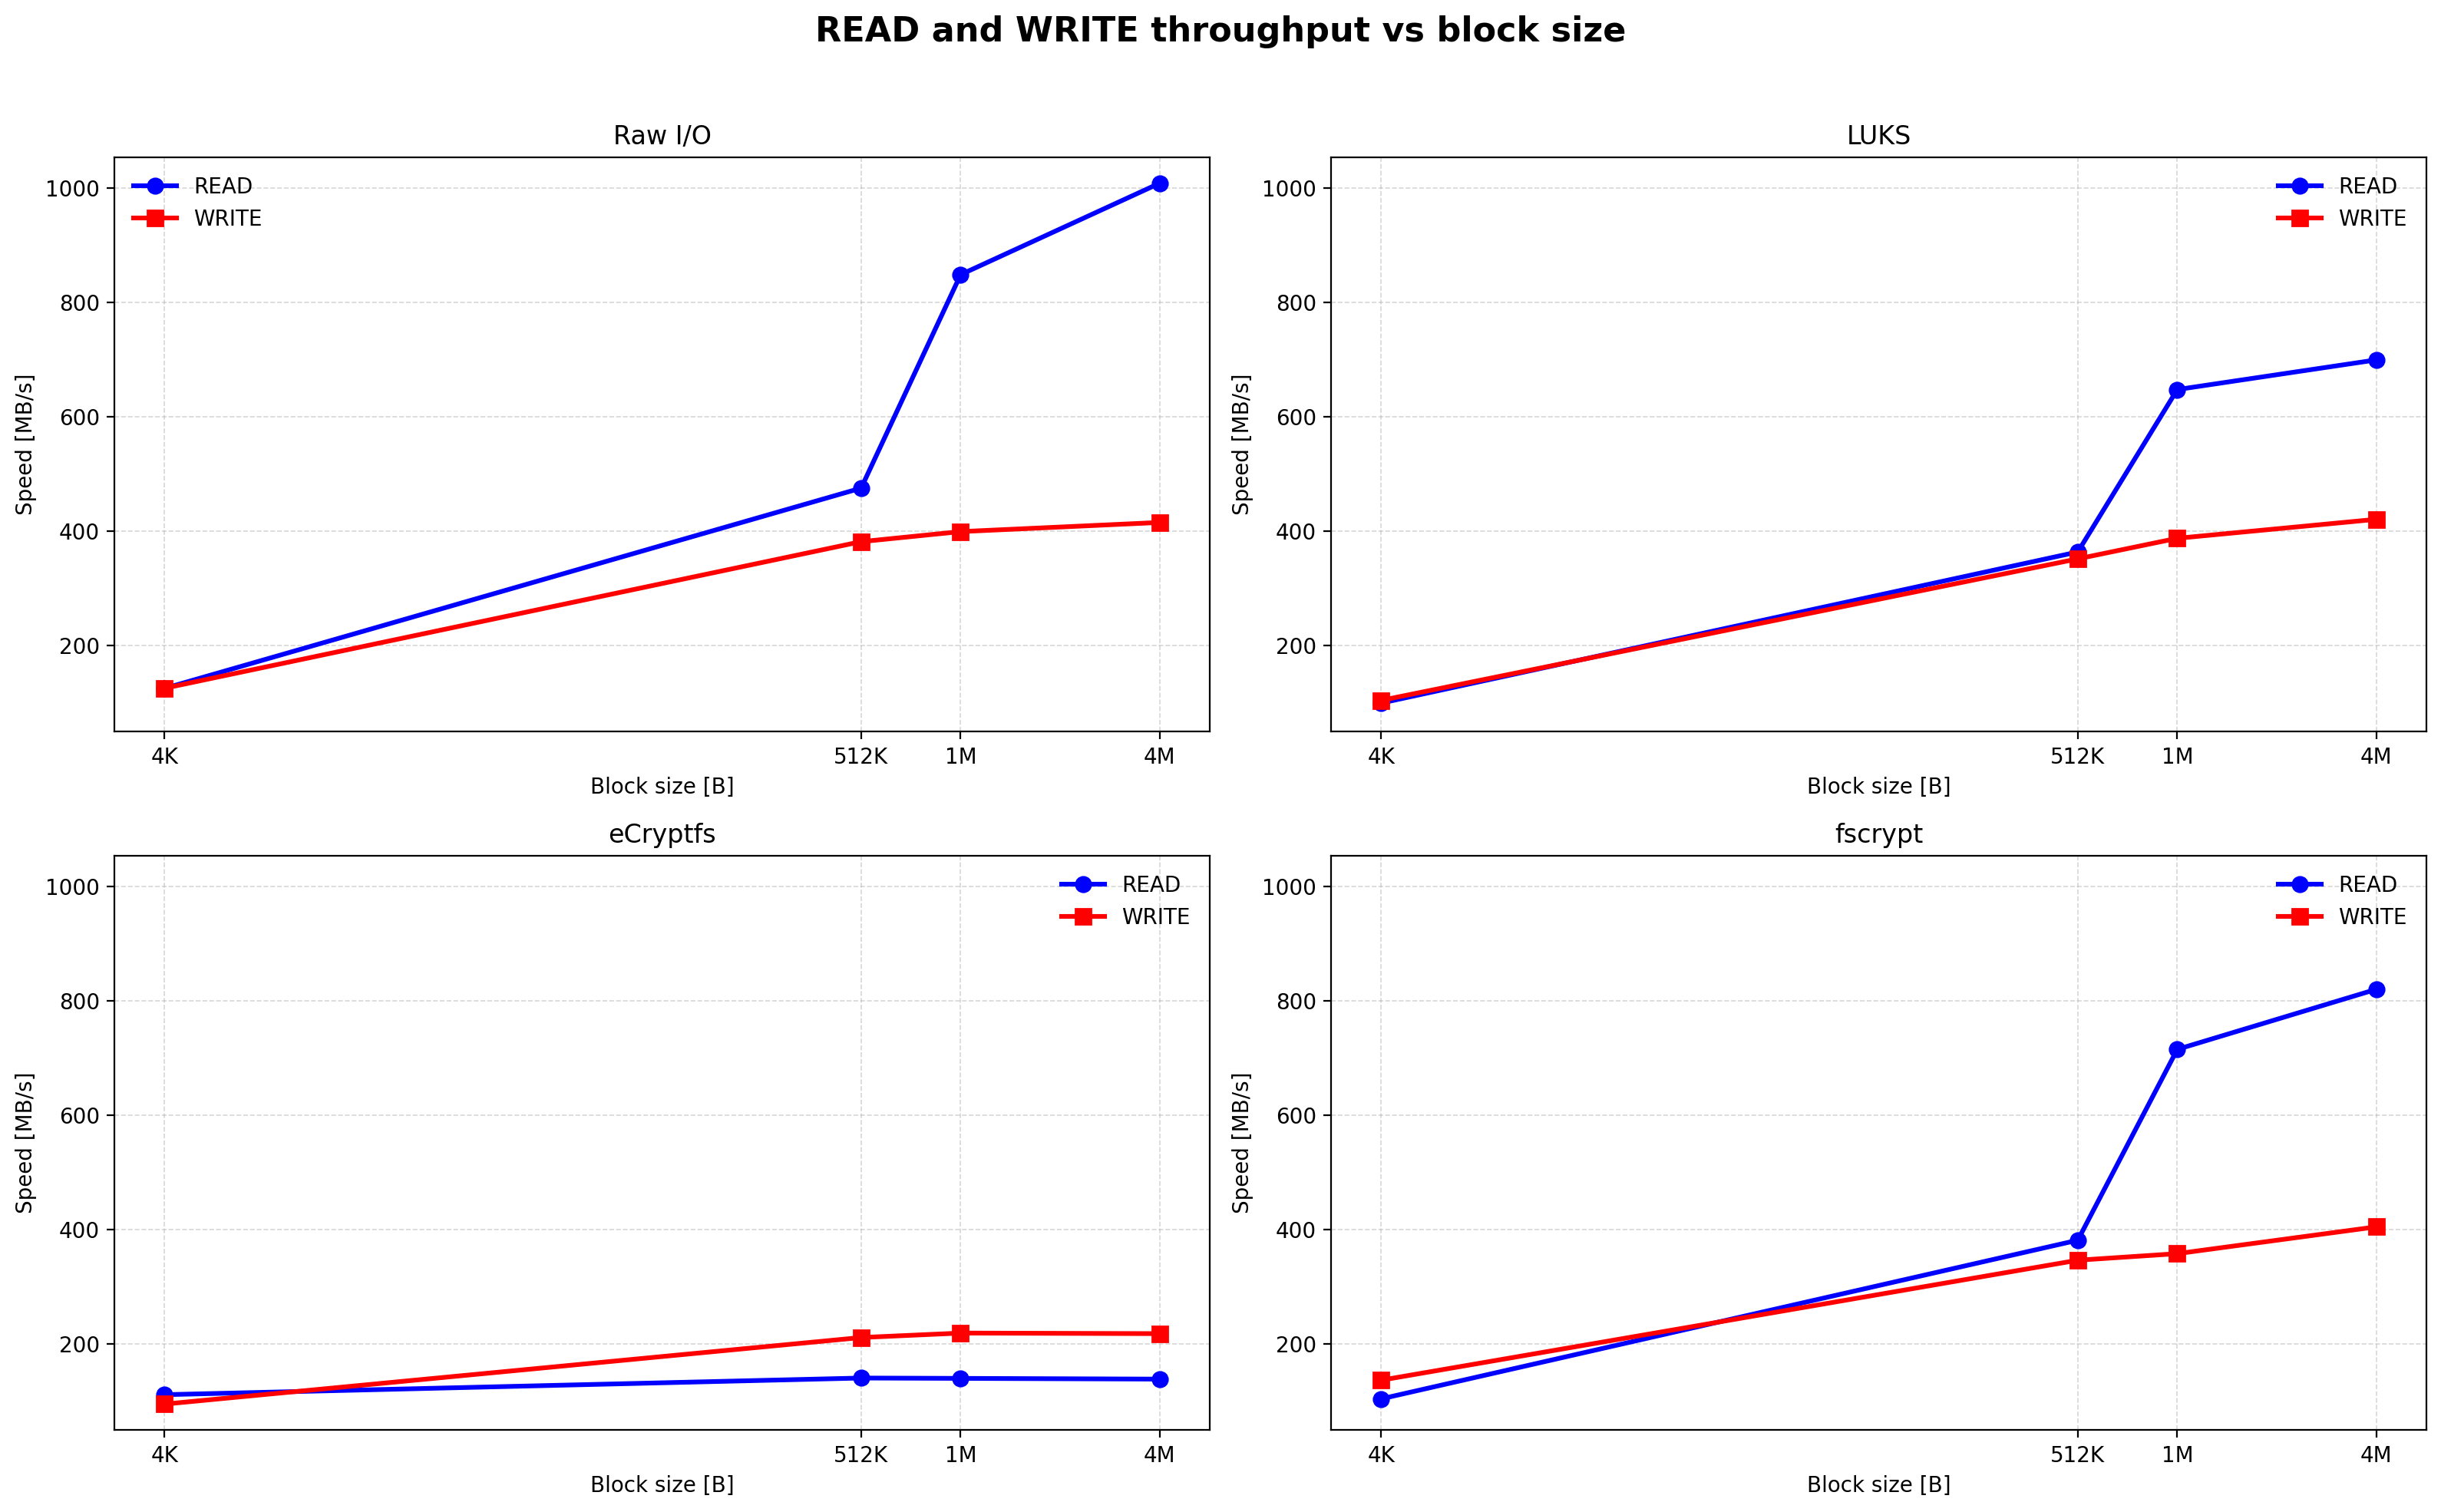
\includegraphics[width=\linewidth]{dd_final_plot.png}
    \caption{Wykres zależności wielkości bloku w bajtach do szybkości operacji kopiowania z
    oraz do szyfrowanych plików różnymi mechanizmami.}
    \label{fig:dd_results}
\end{figure}

\subsubsection{Wnioski}

Na podstawie surowych danych z tabeli \eqref{tab:dd_results} oraz wykresu \eqref{fig:dd_results},
można stwierdzić, że najlepsze wyniki dla czytania danych osiąga brak szyfrowania.
LUKS oraz fscrypt osiągają porównywalne wyniki, co wynika ze sposobu szyfrowania, gdzie
dla LUKS szyfrowana jest cała partycja, oraz dla fscrypt, gdzie szyfrowane są katalogi, co
powoduje niewielki narzut na szybkość odczytywania danych w porównaniu do braku szyfrowania.
W przypadku eCryptfs, gdzie szyfrowanie odbywa się per-plik, narzut na operacje czytania
jest największy ze wszystkich porównywanych mechanizmów.

Mechanizmy LUKS oraz fscrypt w porównaniu do braku szyfrowania nie powodują dodatkowego narzutu,
związanego z zapisem danych do plików. Natomiast podobnie jak dla operacji odczytu,
eCryptfs powoduje zauważalny spadek w szybkości zapisów w porównaniu do pozostałych metod
szyfrowania.


\subsection{Testy wykorzystujące \texttt{fio}}
Narzędzie \texttt{fio} pozwala na bardziej złożone testy wydajności wybranego mechanizmu
szyfrowania plików dzięki jednoczesnym operacjom wejścia i wyjścia oraz na między innymi
wybranie sposobu kopiowania plików (sekwencyjne \& losowe). W ramach benchmarków
przetestowano kopiowanie sekwencyjne i losowe bloków o różnej wielkości oraz
jednoczesne wykonywanie operacji I/O o równym (50/50) rozłożeniu oraz nierównomiernym (70/30).


\begin{table}[H]
    \centering
    \small
    \begin{tabular}{|l|l|r|r|}
        \hline
        Mechanism & Test & Read I/OPS & Write I/OPS \\
        \hline
        Raw I/O & Sequential write 4k & 0 & 5450 \\
        Raw I/O & Sequential read 4k & 6358 & 0 \\
        Raw I/O & Sequential write 1M & 0 & 1370 \\
        Raw I/O & Sequential read 1M & 1207 & 0 \\
        Raw I/O & Random write 4k & 0 & 3201 \\
        Raw I/O & Random read 4k & 3533 & 0 \\
        Raw I/O & Random write 1M & 0 & 1349 \\
        Raw I/O & Random read 1M & 1193 & 0 \\
        Raw I/O & Mixed 70\%R/30\%W 1M & 839 & 360 \\
        Raw I/O & Mixed 50\%R/50\%W 1M & 605 & 604 \\
        LUKS & Sequential write 4k & 0 & 17167 \\
        LUKS & Sequential read 4k & 6047 & 0 \\
        LUKS & Sequential write 1M & 0 & 1305 \\
        LUKS & Sequential read 1M & 1177 & 0 \\
        LUKS & Random write 4k & 0 & 2853 \\
        LUKS & Random read 4k & 3416 & 0 \\
        LUKS & Random write 1M & 0 & 1343 \\
        LUKS & Random read 1M & 1214 & 0 \\
        LUKS & Mixed 70\%R/30\%W 1M & 894 & 383 \\
        LUKS & Mixed 50\%R/50\%W 1M & 626 & 633 \\
        eCryptfs & Sequential write 4k  & 0 & 114356 \\
        eCryptfs & Sequential read 4k  & 910493 & 0 \\
        eCryptfs & Sequential write 1M  & 0 & 464 \\
        eCryptfs & Sequential read 1M  & 2264 & 0 \\
        eCryptfs & Random write 4k  & 0 & 100559 \\
        eCryptfs & Random read 4k  & 1963 & 0 \\
        eCryptfs & Random write 1M  & 0 & 474 \\
        eCryptfs & Random read 1M  & 17937 & 0 \\
        eCryptfs & Mixed 70\%R/30\%W 1M  & 1108 & 471 \\
        eCryptfs & Mixed 50\%R/50\%W 1M  & 481 & 490 \\
        fscrypt & Sequential write 4k & 0 & 261970 \\
        fscrypt & Sequential read 4k & 2893650 & 0 \\
        fscrypt & Sequential write 1M & 0 & 2105 \\
        fscrypt & Sequential read 1M & 19955 & 0 \\
        fscrypt & Random write 4k & 0 & 280132 \\
        fscrypt & Random read 4k & 2222 & 0 \\
        fscrypt & Random write 1M & 0 & 2459 \\
        fscrypt & Random read 1M & 20678 & 0 \\
        fscrypt & Mixed 70\%R/30\%W 1M & 4330 & 1854 \\
        fscrypt & Mixed 50\%R/50\%W 1M & 1883 & 1878 \\
        \hline
    \end{tabular}
    \caption{Tabela wyników w podziale na operacje I/O (wejścia/wyjścia) na sekundę.}
    \label{tab:fio_iops}
\end{table}

\begin{table}[H]
    \centering
    \small
    \begin{tabular}{|l|l|r|r|}
        \hline
        Mechanism & Test & Read BW MB/s & Write BW MB/s \\
        \hline
        Raw I/O & Sequential write 4k & 0.00 & 21.29 \\
        Raw I/O & Sequential read 4k & 24.83 & 0.00 \\
        Raw I/O & Sequential write 1M & 0.00 & 1369.96 \\
        Raw I/O & Sequential read 1M & 1207.32 & 0.00 \\
        Raw I/O & Random write 4k & 0.00 & 12.50 \\
        Raw I/O & Random read 4k & 13.80 & 0.00 \\
        Raw I/O & Random write 1M & 0.00 & 1349.27 \\
        Raw I/O & Random read 1M & 1193.10 & 0.00 \\
        Raw I/O & Mixed 70\%R/30\%W 1M & 839.14 & 360.00 \\
        Raw I/O & Mixed 50\%R/50\%W 1M & 604.72 & 603.82 \\
        LUKS & Sequential write 4k & 0.00 & 67.06 \\
        LUKS & Sequential read 4k & 23.62 & 0.00 \\
        LUKS & Sequential write 1M & 0.00 & 1305.19 \\
        LUKS & Sequential read 1M & 1176.68 & 0.00 \\
        LUKS & Random write 4k & 0.00 & 11.14 \\
        LUKS & Random read 4k & 13.34 & 0.00 \\
        LUKS & Random write 1M & 0.00 & 1342.88 \\
        LUKS & Random read 1M & 1213.72 & 0.00 \\
        LUKS & Mixed 70\%R/30\%W 1M & 893.97 & 383.48 \\
        LUKS & Mixed 50\%R/50\%W 1M & 626.13 & 632.52 \\
        eCryptfs & Sequential write 4k  & 0.00 & 446.70 \\
        eCryptfs & Sequential read 4k  & 3556.61 & 0.00 \\
        eCryptfs & Sequential write 1M  & 0.00 & 464.01 \\
        eCryptfs & Sequential read 1M  & 2263.98 & 0.00 \\
        eCryptfs & Random write 4k  & 0.00 & 392.81 \\
        eCryptfs & Random read 4k  & 7.67 & 0.00 \\
        eCryptfs & Random write 1M  & 0.00 & 473.64 \\
        eCryptfs & Random read 1M  & 17937.47 & 0.00 \\
        eCryptfs & Mixed 70\%R/30\%W 1M  & 1108.41 & 470.83 \\
        eCryptfs & Mixed 50\%R/50\%W 1M  & 481.25 & 489.98 \\
        fscrypt & Sequential write 4k & 0.00 & 1023.32 \\
        fscrypt & Sequential read 4k & 11303.32 & 0.00 \\
        fscrypt & Sequential write 1M & 0.00 & 2105.25 \\
        fscrypt & Sequential read 1M & 19955.23 & 0.00 \\
        fscrypt & Random write 4k & 0.00 & 1094.27 \\
        fscrypt & Random read 4k & 8.68 & 0.00 \\
        fscrypt & Random write 1M & 0.00 & 2458.55 \\
        fscrypt & Random read 1M & 20677.51 & 0.00 \\
        fscrypt & Mixed 70\%R/30\%W 1M & 4330.03 & 1853.64 \\
        fscrypt & Mixed 50\%R/50\%W 1M & 1883.16 & 1877.72 \\
        \hline
    \end{tabular}
    \caption{Tabela wyników przepustowości osiągana przez poszczególne mechanizmy szyfrowania.}
    \label{tab:fio_bw}
\end{table}

\begin{table}[H]
    \centering
    \small
    \begin{tabular}{|l|l|r|r|}
        \hline
        Mechanism & Test & Read latency us & Write latency us \\
        \hline
        Raw I/O & Sequential write 4k & 0.0 & 11736.5 \\
        Raw I/O & Sequential read 4k & 10060.9 & 0.0 \\
        Raw I/O & Sequential write 1M & 0.0 & 46686.5 \\
        Raw I/O & Sequential read 1M & 52939.3 & 0.0 \\
        Raw I/O & Random write 4k & 0.0 & 19985.0 \\
        Raw I/O & Random read 4k & 18106.7 & 0.0 \\
        Raw I/O & Random write 1M & 0.0 & 47402.1 \\
        Raw I/O & Random read 1M & 53592.4 & 0.0 \\
        Raw I/O & Mixed 70\%R/30\%W 1M & 38852.4 & 87042.6 \\
        Raw I/O & Mixed 50\%R/50\%W 1M & 33539.9 & 72302.3 \\
        LUKS & Sequential write 4k & 0.0 & 3726.9 \\
        LUKS & Sequential read 4k & 10576.6 & 0.0 \\
        LUKS & Sequential write 1M & 0.0 & 49017.9 \\
        LUKS & Sequential read 1M & 54339.2 & 0.0 \\
        LUKS & Random write 4k & 0.0 & 22427.3 \\
        LUKS & Random read 4k & 18725.6 & 0.0 \\
        LUKS & Random write 1M & 0.0 & 47646.6 \\
        LUKS & Random read 1M & 52681.0 & 0.0 \\
        LUKS & Mixed 70\%R/30\%W 1M & 40498.3 & 72345.9 \\
        LUKS & Mixed 50\%R/50\%W 1M & 32301.8 & 69139.9 \\
        eCryptfs & Sequential write 4k  & 0.0 & 558.9 \\
        eCryptfs & Sequential read 4k  & 69.7 & 0.0 \\
        eCryptfs & Sequential write 1M  & 0.0 & 137588.8 \\
        eCryptfs & Sequential read 1M  & 28107.0 & 0.0 \\
        eCryptfs & Random write 4k  & 0.0 & 605.6 \\
        eCryptfs & Random read 4k  & 32573.9 & 0.0 \\
        eCryptfs & Random write 1M  & 0.0 & 128480.3 \\
        eCryptfs & Random read 1M  & 3542.3 & 0.0 \\
        eCryptfs & Mixed 70\%R/30\%W 1M  & 38011.3 & 45616.1 \\
        eCryptfs & Mixed 50\%R/50\%W 1M  & 61994.8 & 69244.7 \\
        fscrypt & Sequential write 4k & 0.0 & 243.9 \\
        fscrypt & Sequential read 4k & 21.9 & 0.0 \\
        fscrypt & Sequential write 1M & 0.0 & 29404.3 \\
        fscrypt & Sequential read 1M & 3203.1 & 0.0 \\
        fscrypt & Random write 4k & 0.0 & 182.2 \\
        fscrypt & Random read 4k & 28784.9 & 0.0 \\
        fscrypt & Random write 1M & 0.0 & 25881.3 \\
        fscrypt & Random read 1M & 3088.4 & 0.0 \\
        fscrypt & Mixed 70\%R/30\%W 1M & 10190.6 & 10668.3 \\
        fscrypt & Mixed 50\%R/50\%W 1M & 17036.1 & 16927.0 \\
        \hline
    \end{tabular}
    \caption{Tabela wyników opóźnienia odczytu i zapisu mierzone w mikrosekundach.}
    \label{tab:fio_latency}
\end{table}

\begin{table}[H]
    \centering
    \small
    \begin{tabular}{|l|l|r|r|}
        \hline
        Mechanism & Test & CPU user \% & CPU sys \% \\
        \hline
        Raw I/O & Sequential write 4k & 0.3 & 47.2 \\
        Raw I/O & Sequential read 4k & 0.3 & 57.2 \\
        Raw I/O & Sequential write 1M & 1.1 & 41.8 \\
        Raw I/O & Sequential read 1M & 0.2 & 31.2 \\
        Raw I/O & Random write 4k & 0.2 & 34.5 \\
        Raw I/O & Random read 4k & 0.2 & 26.5 \\
        Raw I/O & Random write 1M & 1.1 & 41.0 \\
        Raw I/O & Random read 1M & 0.2 & 31.1 \\
        Raw I/O & Mixed 70\%R/30\%W 1M & 0.5 & 41.5 \\
        Raw I/O & Mixed 50\%R/50\%W 1M & 0.7 & 43.7 \\
        LUKS & Sequential write 4k & 0.9 & 6.5 \\
        LUKS & Sequential read 4k & 0.2 & 56.2 \\
        LUKS & Sequential write 1M & 1.0 & 4.2 \\
        LUKS & Sequential read 1M & 0.3 & 20.9 \\
        LUKS & Random write 4k & 0.2 & 5.8 \\
        LUKS & Random read 4k & 0.2 & 22.5 \\
        LUKS & Random write 1M & 1.0 & 3.8 \\
        LUKS & Random read 1M & 0.3 & 22.4 \\
        LUKS & Mixed 70\%R/30\%W 1M & 0.6 & 23.4 \\
        LUKS & Mixed 50\%R/50\%W 1M & 0.7 & 21.3 \\
        eCryptfs & Sequential write 4k  & 3.3 & 87.1 \\
        eCryptfs & Sequential read 4k  & 13.3 & 58.6 \\
        eCryptfs & Sequential write 1M  & 0.5 & 85.1 \\
        eCryptfs & Sequential read 1M  & 0.7 & 46.4 \\
        eCryptfs & Random write 4k  & 2.1 & 72.8 \\
        eCryptfs & Random read 4k  & 1.0 & 6.3 \\
        eCryptfs & Random write 1M  & 0.7 & 77.5 \\
        eCryptfs & Random read 1M  & 0.9 & 92.0 \\
        eCryptfs & Mixed 70\%R/30\%W 1M  & 0.9 & 80.3 \\
        eCryptfs & Mixed 50\%R/50\%W 1M  & 0.9 & 83.0 \\
        fscrypt & Sequential write 4k & 4.1 & 25.3 \\
        fscrypt & Sequential read 4k & 18.0 & 70.0 \\
        fscrypt & Sequential write 1M & 1.7 & 27.7 \\
        fscrypt & Sequential read 1M & 3.0 & 90.8 \\
        fscrypt & Random write 4k & 3.3 & 25.0 \\
        fscrypt & Random read 4k & 0.3 & 23.5 \\
        fscrypt & Random write 1M & 2.0 & 28.0 \\
        fscrypt & Random read 1M & 2.2 & 95.2 \\
        fscrypt & Mixed 70\%R/30\%W 1M & 1.4 & 28.1 \\
        fscrypt & Mixed 50\%R/50\%W 1M & 1.5 & 28.7 \\
        \hline
    \end{tabular}
    \caption{Tabela wykorzystania CPU w testach.}
    \label{tab:fio_cpu}
\end{table}

\begin{figure}[H]
    \centering
    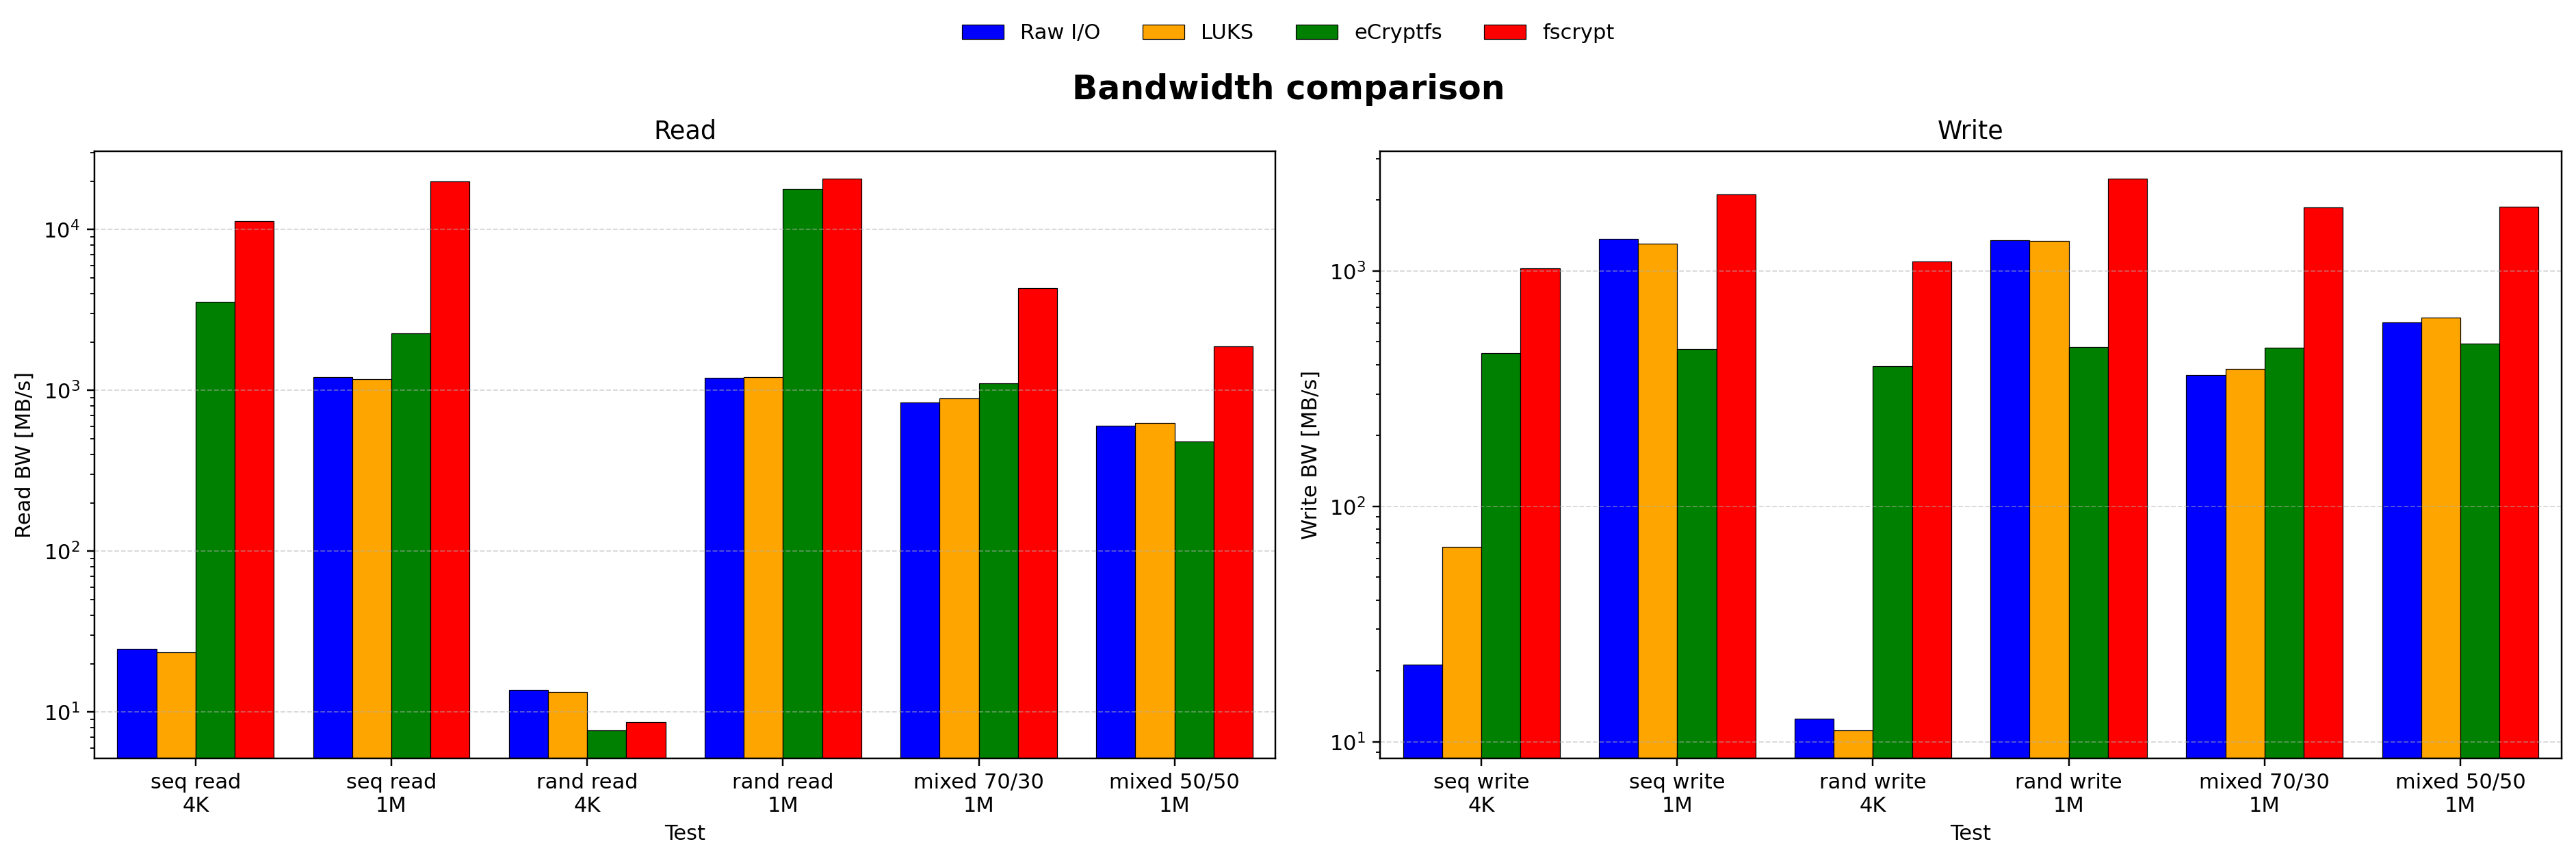
\includegraphics[width=\linewidth]{fio_summary_plots/fio_summary_bandwidth.png}
    \caption{Wykres przepustowości poszczególnych mechanizmów szyfrowania dla kolejnych
    testów wydajności.}
    \label{fig:fio_bandwidth}
\end{figure}

\begin{figure}[H]
    \centering
    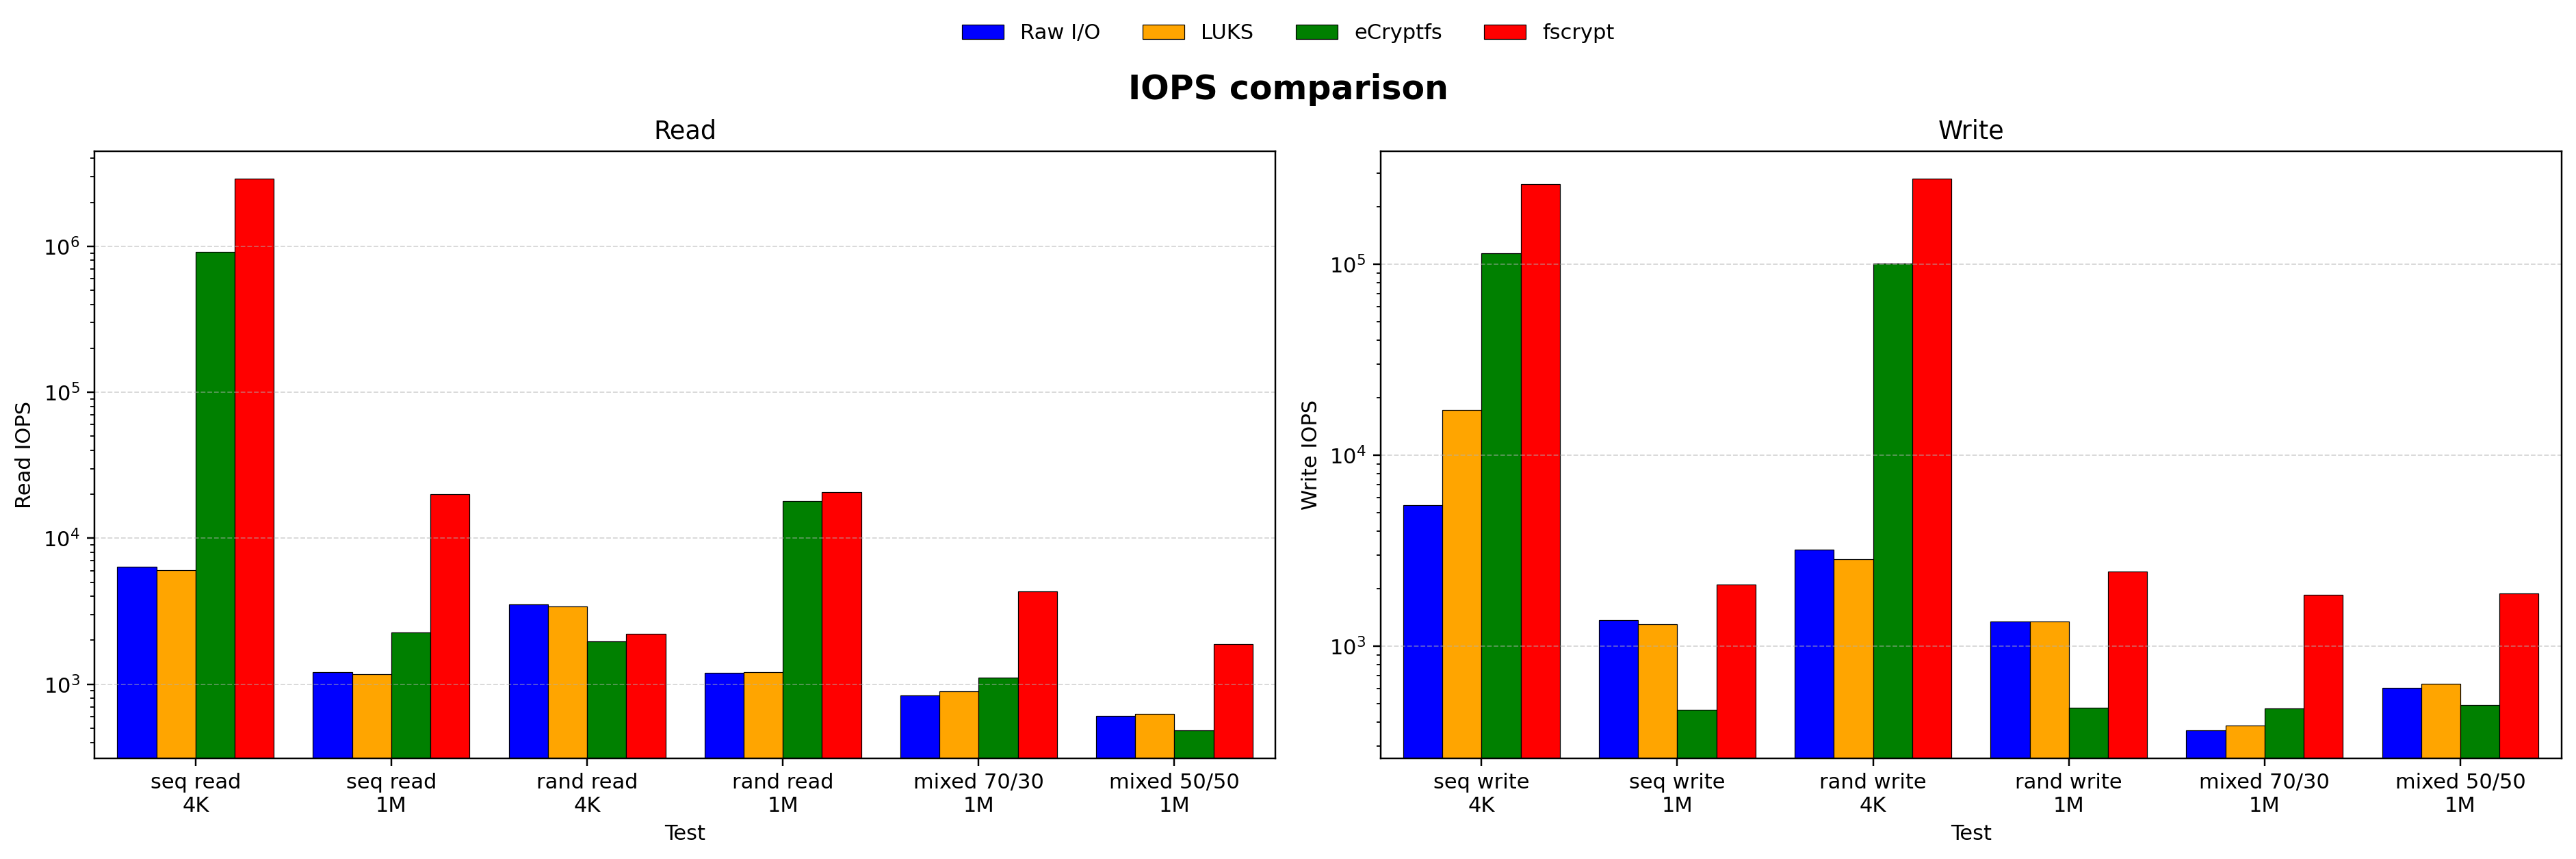
\includegraphics[width=\linewidth]{fio_summary_plots/fio_summary_iops.png}
    \caption{Wykres ilości operacji wejścia i wyjścia na sekundę poszczególnych mechanizmów
    szyfrowania dla kolejnych testów wydajności.}
    \label{fig:fio_iops}
\end{figure}

\begin{figure}[H]
    \centering
    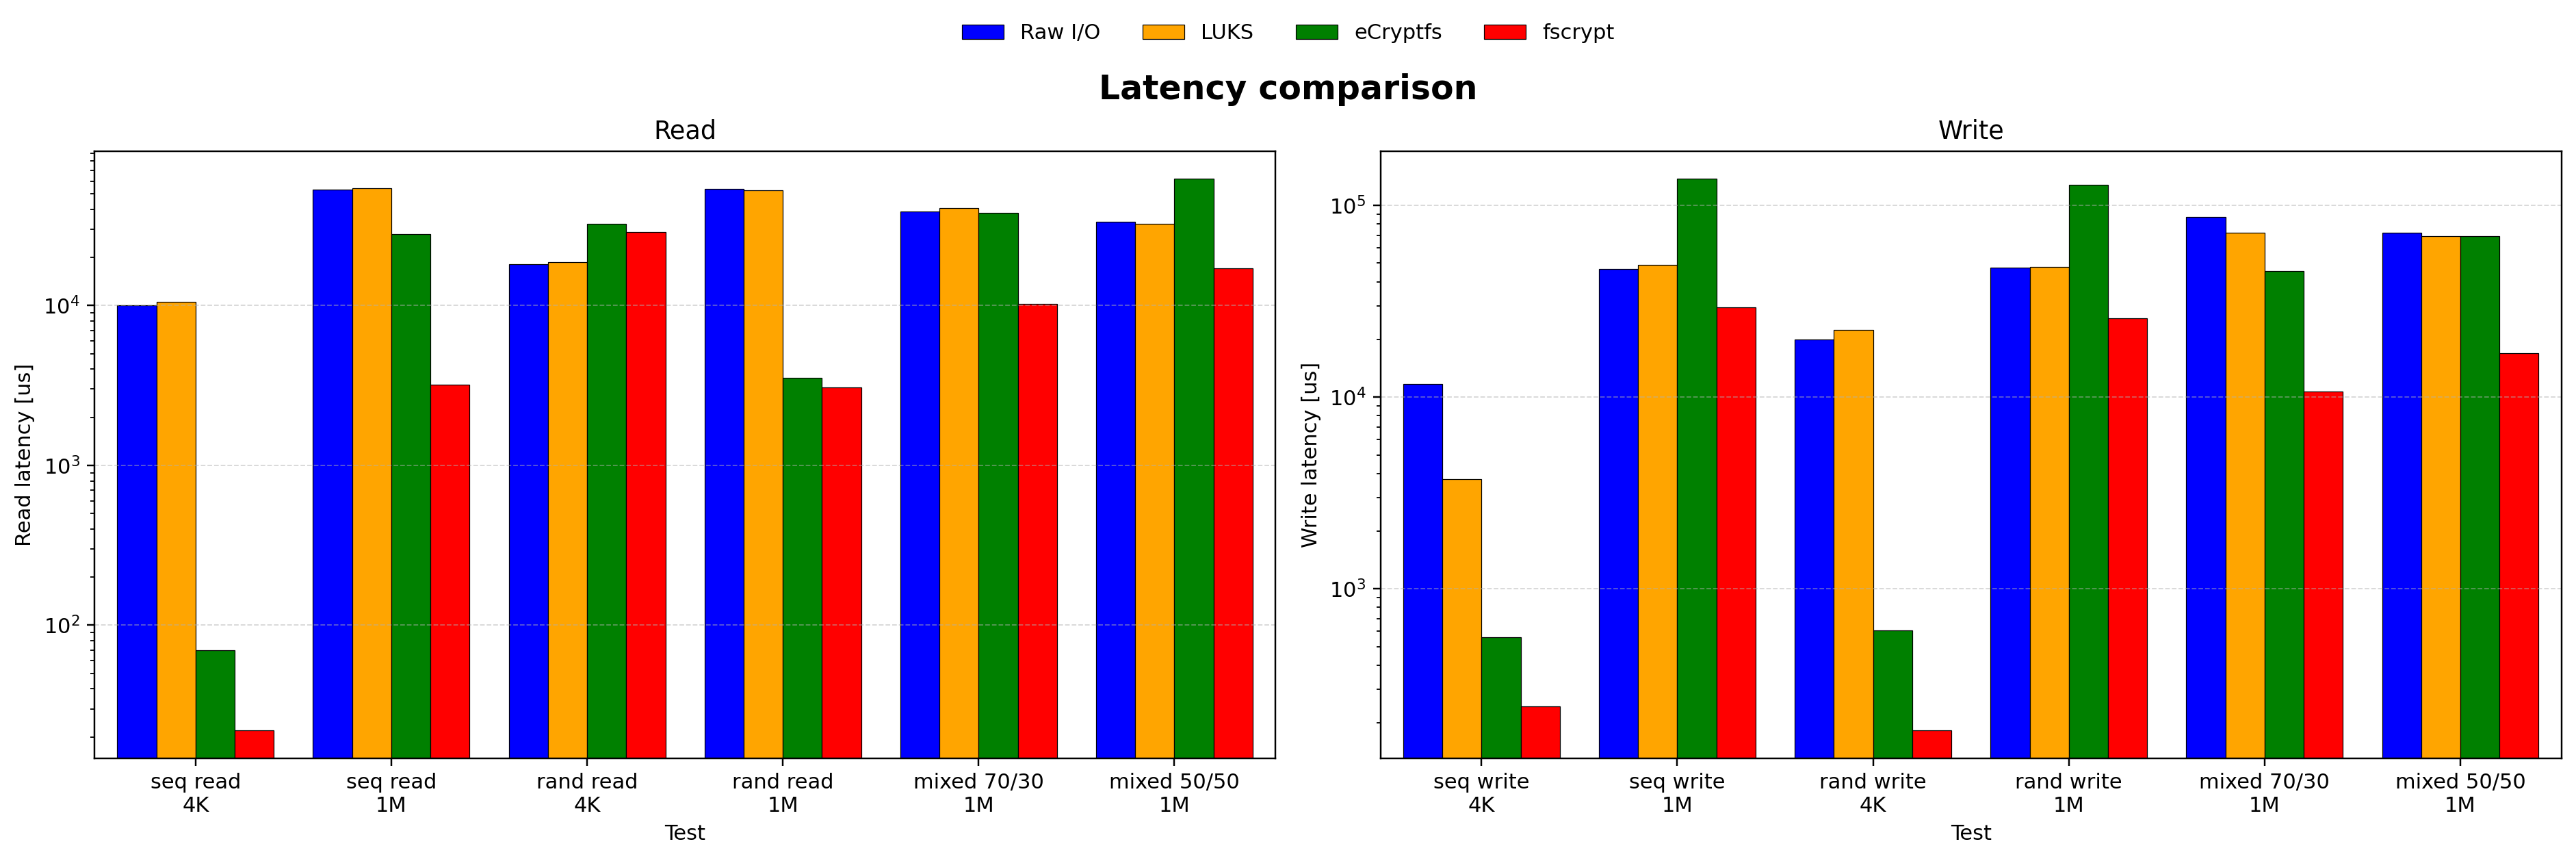
\includegraphics[width=\linewidth]{fio_summary_plots/fio_summary_latency.png}
    \caption{Wykres opóźnienia dla poszczególnych mechanizmów szyfrowania dla kolejnych testów
    wydajności.}
    \label{fig:fio_latency}
\end{figure}

\begin{figure}[H]
    \centering
    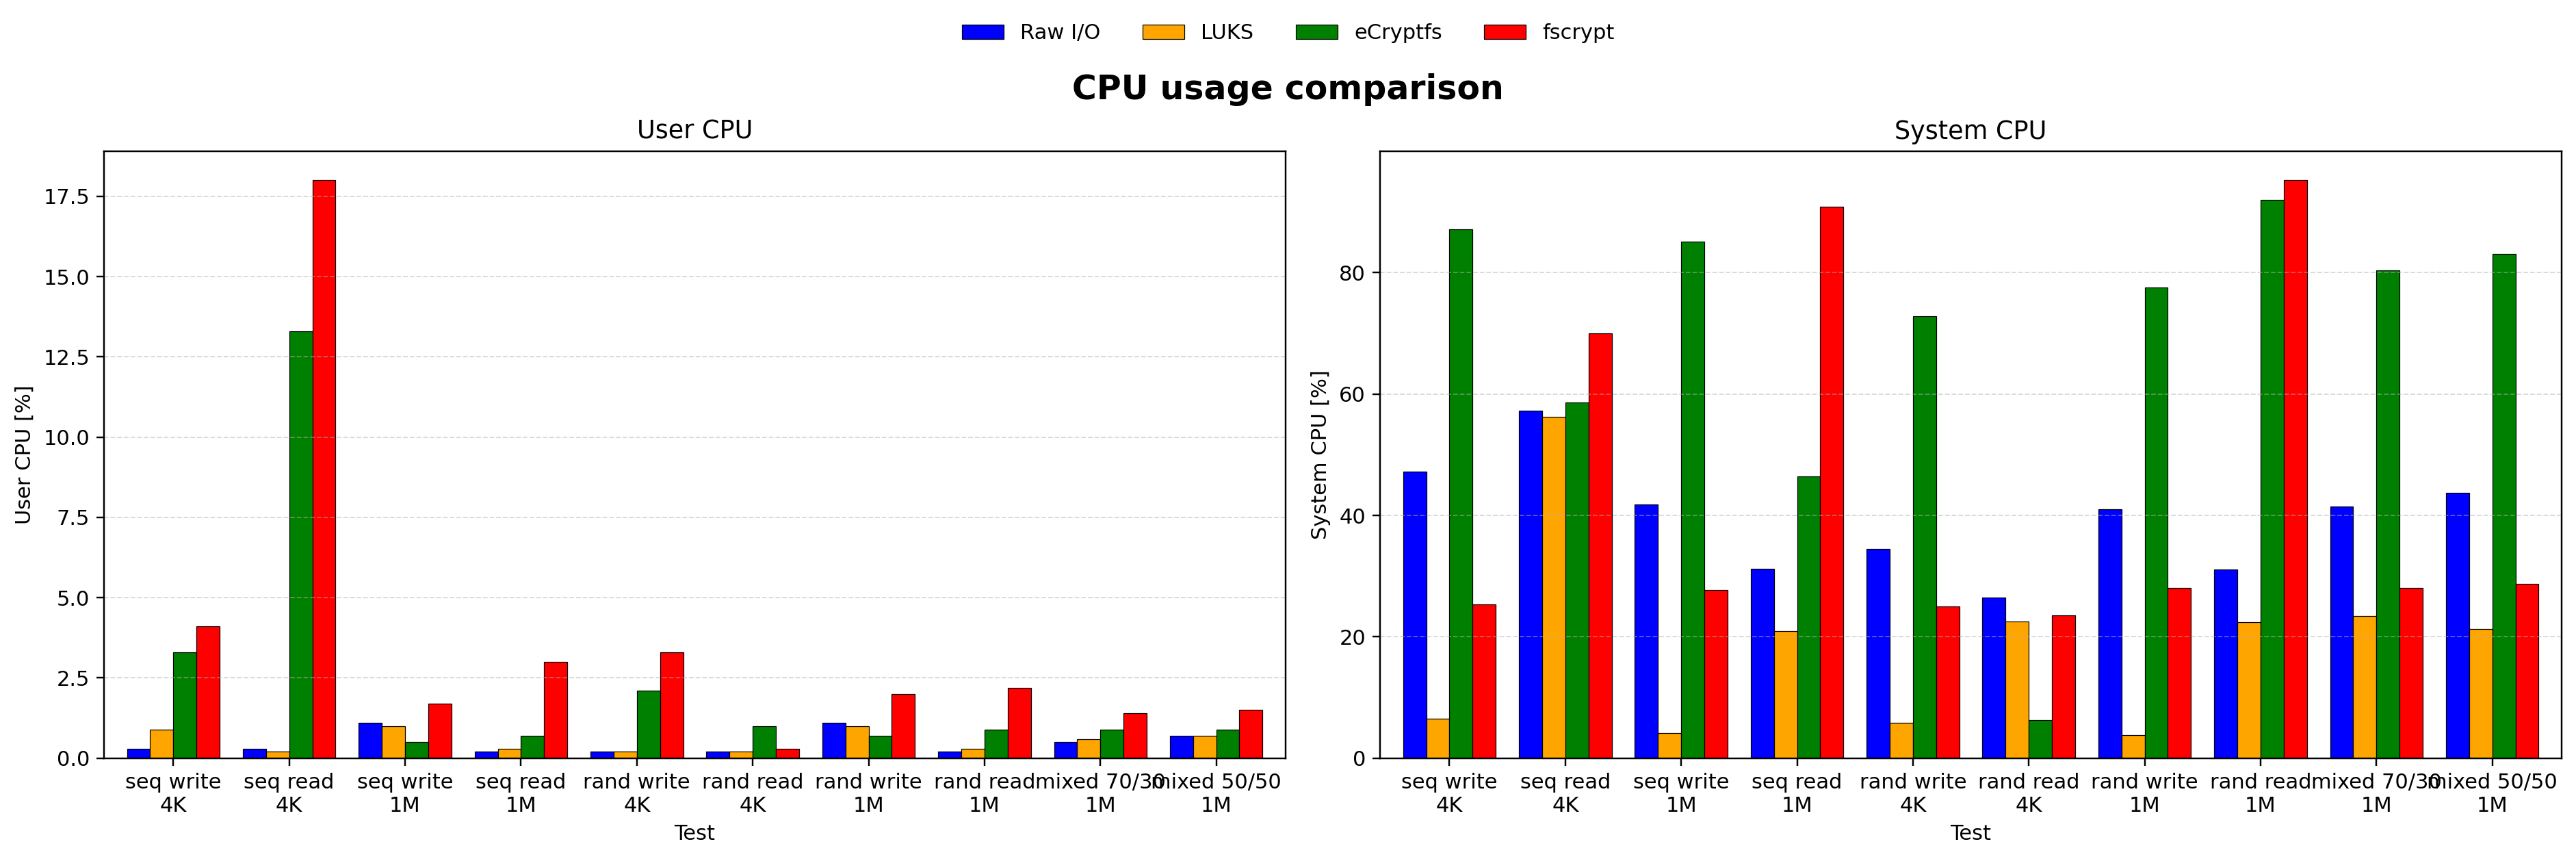
\includegraphics[width=\linewidth]{fio_summary_plots/fio_summary_cpu.png}
    \caption{Wykres zużycia zasobów CPU dla poszczególnych mechanizmów szyfrowania dla kolejnych
    testów wydajności.}
    \label{fig:fio_cpu}
\end{figure}

\subsubsection{Wnioski}

W przypadku wyników otrzymanych dla fscrypt oraz eCryptfs, warto zwrócić uwagę na wykorzystanie
pamięci podręcznej w testach. Pomimo zastosowania flagi \texttt{invalidate=1} w konfiguracji
testów \texttt{fio} oraz czyszczenia bufora jądra przed każdym uruchomieniem benchmarku przy
użyciu poleceń \texttt{sync} oraz \texttt{echo 3 > /proc/sys/vm/drop\_caches}, wyniki dla
fscrypt i eCryptfs wskazują na silny wpływ pamięci RAM.
Dla fscrypt i eCryptfs odczyt danych osiąga przepustowość rzędu kilku, bądź kilkunastu
gigabajtow na sekundę. Otrzymane wartości znacznie przewyższają możliwości wykorzystanego
dysku SSD (około 1200 MB/s dla operacji bez szyfrowania). Wartości rzędu kilkunastu GB na
sekundę wskazują, na przechowywanie danych w pamięci RAM oraz bezpośredni z niej odczyt.

Natomiast wyniki otrzymane dla LUKS są bardzo zbliżone do wyników bez szyfrowania. Warto
zauważyć, że zużycie CPU jest bardzo niskie w trybie systemowym w porównaniu do pozostałych
metod szyfrowania. W testach mieszanych (70\%R/30\%W oraz 50\%R/50\%W), LUKS i brak szyfrowania
osiągają zbliżone wyniki w granicach, co potwierdza spójność wyników dla tego mechanizmu.

\subsection{Podsumowanie}
Wyniki benchmarków pozwalają stwierdzić, że LUKS jest mechanizmem szyfrowania o najmniejszym
narzucie porównując z wydajnością bez szyfrowania, przy jednoczesnym bardzo niskim zużyciu CPU.
eCryptfs niesie za sobą znaczący narzut obliczeniowy (CPU sys powyżej 80\%) oraz obniżoną
przepustowość dla dużych operacji, pomimo że wyniki dla małych bloków są zawyżone na wskutek
buforowania danych. Wyniki fscrypt w zakresie operacji odczytu są silnie powiązane z
wykorzystaniem pamięci cache i nie odzwierciedlają wydajności dyskowej. Jedynie wyniki zapisu
oraz losowego odczytu przedstawiają realne osiągi oraz wydajność mechanizmu.
Mimo zastosowania sposobów czyszczenia pamięci podręcznej, fscrypt skutecznie
ponownie wypełnia cache podczas operacji, co uniemożliwia wiarygodny pomiar wydajności
dyskowej dla tego mechanizmu w zastosowanej konfiguracji testów.


\paragraph{Operacje na małych blokach (4K) kontra dużych blokach (1M).}
We wszystkich mechanizmach przepustowość wyrażona w MB/s dla bloków 4K jest drastycznie
niższa niż dla bloków 1M, co wynika z dominacji opóźnienia dyskowego przy małych operacjach.
Dla braku szyfrowania, sekwencyjny zapis 4K daje wyniki rzędu kilkudziesięciu megabajtów na
sekundę, podczas gdy dla 1M osiąga wartości ponad gigabajt na sekundę. LUKS zachowuje tę
proporcję, natomiast fscrypt i eCryptfs wykazują tutaj użycie pamięci podręcznej i nie
odzwierciedlają rzeczywistej wydajności dyskowej.


\section{Rekomendacje dla scenariuszy użycia}

Poniższe rekomendacje użycia poszczególnych mechanizmów szyfrowania oparte są na
otrzymanych wynikach wydajności oraz na podstawie charakterystyk poszczególnych metod oraz
modeli zagrożeń.

\subsection{Szyfrowanie dysku systemowego lub partycji danych}

Rekomendowanym rozwiązaniem jest LUKS. Szyfrowanie na poziomie urządzenia blokowego
zapewnia transparentną ochronę całej partycji, w tym systemu plików, metadanych, struktury
katalogów i danych. Wyniki benchmarków potwierdzają, że LUKS wprowadza minimalny narzut
wydajnościowy zarówno dla operacji sekwencyjnych, jak i losowych. Osiągi dla bloków 1M
są praktycznie identyczne z wynikami bez szyfrowania. Zużycie CPU w trybie systemowym
jest przy tym znacząco niższe niż w przypadku pozostałych mechanizmów. LUKS jest standardowym
i aktywnie wspieranym rozwiązaniem w ekosystemie Linux, zalecanym dla pełnego szyfrowania dysku
laptopów, stacji roboczych oraz serwerów.

\subsection{Szyfrowanie katalogu domowego użytkownika}

Rekomendowanym rozwiązaniem jest fscrypt. W odróżnieniu od LUKS, fscrypt pozwala
na szyfrowanie na poziomie katalogu, co umożliwia niezależne szyfrowanie przestrzeni
różnych użytkowników bez konieczności tworzenia oddzielnych partycji. fscrypt jest natywnie
zintegrowany z popularnymi systemami plików (ext4, f2fs, UBIFS) i aktywnie rozwijany.
W testach \texttt{dd} wyniki zapisu dla fscrypt są zbliżone do LUKS i operacji bez szyfrowania
dla większych bloków. Rozwiązanie to zastępuje przestarzały eCryptfs, który od 2016 roku nie
jest aktywnie rozwijany i został wycofany przez Ubuntu jako domyślny mechanizm szyfrowania
katalogów domowych.

\subsection{Środowiska wielodostępne i szyfrowanie selektywne}

W środowiskach, w których różni użytkownicy powinni mieć dostęp wyłącznie do własnych
danych, rekomendowanym rozwiązaniem jest fscrypt. Mechanizm ten pozwala na niezależne
zarządzanie kluczami dla poszczególnych katalogów, a ochrona dostępu realizowana jest przez
standardowe mechanizmy kontroli dostępu systemu Linux takich jak uprawnienia plików. Każdy
użytkownik może posiadać własny klucz szyfrujący, a dane są dostępne wyłącznie po jego dodaniu.
LUKS w tym scenariuszu wymagałby tworzenia oddzielnych partycji dla każdego użytkownika,
co jest rozwiązaniem mniej elastycznym i wprowadza niepotrzebny narzut.

\subsection{Ochrona pojedynczych plików lub przenośnych nośników danych}

W scenariuszu wymagającym przenoszenia zaszyfrowanych plików między różnymi systemami
bez wspólnej infrastruktury kluczy, eCryptfs oferuje unikalną właściwość: metadane
kryptograficzne przechowywane są w nagłówku każdego pliku, co pozwala na odszyfrowanie
pojedynczego pliku na dowolnym systemie posiadającym odpowiedni klucz główny. Należy jednak
uwzględnić istotne ograniczenia tego rozwiązania, takie jak znaczący narzut obliczeniowy,
obniżoną przepustowość dla dużych operacji, czy skrócenie maksymalnej długości nazwy pliku do
143 bajtów. W przypadkach, gdzie pliki nie będą aktywnie przenoszone, zalecany jest wybór fscrypt
lub LUKS.


\section{Podsumowanie}

Przeprowadzona analiza porównawcza trzech mechanizmów szyfrowania danych dostępnych
w systemach Linux LUKS, eCryptfs oraz fscrypt wykazała istotne różnice zarówno pod względem
wydajnościowym, jak i modelu bezpieczeństwa oferowanego przez każde z rozwiązań.
\\\\
Testy z wykorzystaniem \texttt{dd} wykazały, że LUKS oraz fscrypt osiągają wyniki zbliżone
do operacji bez szyfrowania dla bloków większych od 512K. Narzut wydajnościowy
obu mechanizmów jest minimalny, przy czym LUKS charakteryzuje się najniższym zużyciem CPU
w trybie systemowym spośród wszystkich porównywanych metod. eCryptfs jako jedyny mechanizm
wykazuje wyraźny spadek przepustowości we wszystkich testach \texttt{dd}.

Wyniki testów \texttt{fio} potwierdzają dominację LUKS pod względem spójności wyników
z bazowym pomiarem bez szyfrowania. Wartości przepustowości i opóźnień dla LUKS pozostają
na poziomie bliskim wyników czystego systemu plików. W przypadku eCryptfs odnotowano wysokie
obciążenie CPU (powyżej 80\% sys) oraz znaczne opóźnienia przy operacjach na dużych blokach.
Wyniki fscrypt i eCryptfs w zakresie operacji odczytu są silnie zakłócone przez buforowanie
danych w pamięci RAM, co uniemożliwia wiarygodny pomiar rzeczywistej wydajności dyskowej dla
tych mechanizmów w zastosowanej konfiguracji testów.
\\\\
Wszystkie trzy mechanizmy zapewniają ochronę poufności danych w scenariuszach ataków offline.
LUKS chroni całą partycję, w tym metadane systemu plików i strukturę katalogów. fscrypt
i eCryptfs chronią zawartość plików oraz opcjonalnie ich nazwy, lecz nie metadane systemu
plików (rozmiary, uprawnienia, znaczniki czasu). Żaden z analizowanych mechanizmów nie
zapewnia ochrony przed atakami online z uprawnieniami root ani  gdy zaszyfrowane pliki są
zamontowane lub dostępne.

Spośród analizowanych mechanizmów LUKS pozostaje optymalnym wyborem pod kątem stosunku
wydajności do bezpieczeństwa w zastosowaniach ogólnych. fscrypt stanowi nowoczesną
alternatywę tam, gdzie wymagana jest granularność szyfrowania na poziomie katalogu.
eCryptfs, mimo unikalnych właściwości, jest rozwiązaniem przestarzałym i powinien być
stosowany wyłącznie w przypadkach, gdy jego specyficzne cechy są bezwzględnie wymagane.


\end{document}
